\begin{figure*}
\centering
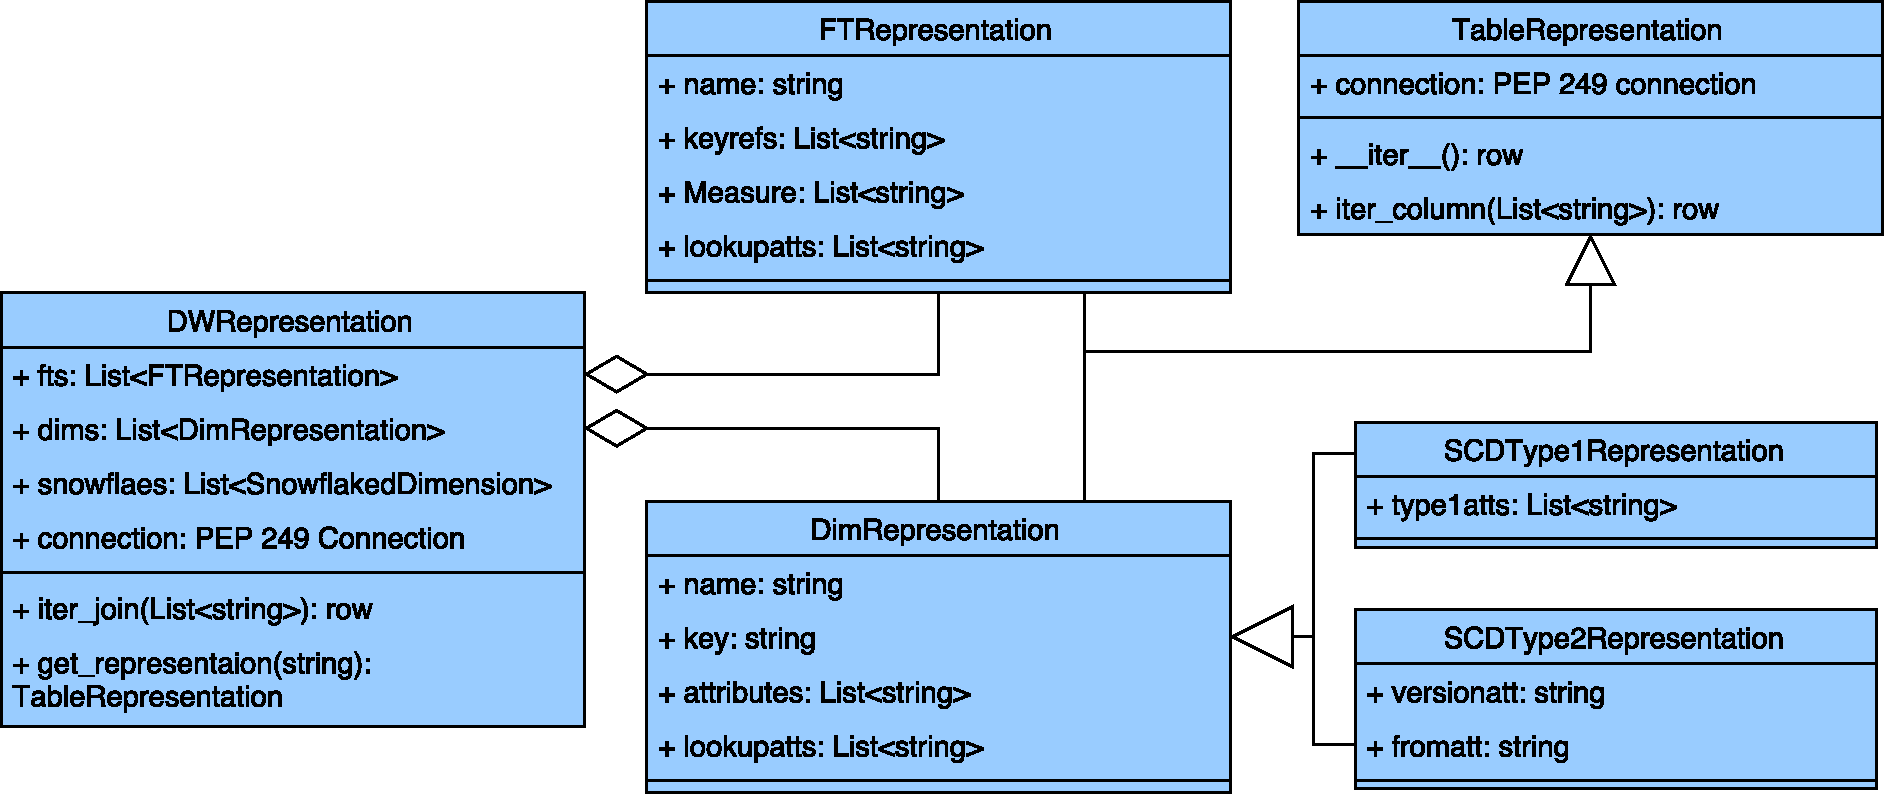
\includegraphics[width=0.9\textwidth]{figures/dwrep_uml.pdf}
\caption{UML diagram of the intermediate representations}
\label{fig:dwrep}
\end{figure*}

\section{Intermediate Data Representations}

This section will go into details about the different intermediate data representations used by the predicates. These representations are meant to standardize input to the predicates so that the DW may be easily accessed. There are two main of intermediate data representations, the \textit{DWRepresentation} and the \textit{TableRepresentation}. DWRepresentation represents the DW as a whole, and the TableRepresentation and its subclasses represent the DWs tables. A UML diagram of the intermediate data representations can be seen in \cref{fig:dwrep}.

\subsection{DWRepresentation}
The \textit{DWRepresentation} is a container object and includes information about the DW's schema and contents. A DWRepresentation object is created by the \textit{RepresentationMaker} by aggregating a number of \textit{TableRepresentations}.

The DWRepresentation has the following main attributes:

\begin{description}
\item[Dimensions] List of \textit{DimRepresentations} detailing each dimension in the DW along with their metadata.
\item[FactTables] List of FactTables in the DW.
\item[Snowflakes] List of Snowflaked dimensions, this is used to construct the DW schema.
\item[Connection] A PEP249 connection object for accessing the the DW, so that we may query it for data later on.
\end{description}
The object also provides methods for connecting to, and extracting data from the DW. Data can be extracted in one of two ways. 

By supplying the name of a table to the get\_data\_representation method, it will return the corresponding TableRepresentation object. DWRepresentaion also supplies the iter\_join method. Given this a number of table names as input, it will return an iterable of the join of specified tables. Both of these methods are used regularly by the predicates.

During instantiation the DWRepresentation also constructs the schema for the given DW. This is done using the \_find\_structure method. For each fact table, we register all dimensions, which it may be naturally joined with. That is, an attribute in the fact table’s keyrefs set is the same as the primary key of a dimension. In the case of our snowflaked dimensions, a fact table may only have a foreign key to the snowflake root. Dimensions within snowflakes are the only ones allowed to have a foreign key to other dimensions. Doing this lookup for each fact table we end up with a dictionary, where the keys are fact table names pointing to sets of dimensions. An example would be \{ft:(A,B)\}, which states that the fact table ft has foreign keys to the dimensions A and B. To this dictionary we add the internal reference information of each snowflaked dimension. Thus it also contains keys for dimensions with foreign keys to other dimensions within snowflakes.

\subsection{TableRepresentation}
\textit{TableRepresentation} is a superclass used for representing data from specific tables. Instantiations of its subclasses contains additional information regarding the tables themselves, such as the table name, attributes etc. These are created by extracting information regarding the tables from the scope of the executed pygrametl program as explained in \cref{ssec:Representation}.

The currently supported tables are:

\begin{itemize}
\item Dimension
\item Type 1 Slowly Changing Dimensions
\item Type 2 Slowly Changing Dimensions
\item FactTable
\end{itemize}

Any dimension or fact table found in a pygrametl program is simply represented in a DimensionRepresentation or FactTableRepresentation respectivly. Special subclasses are made for the slowly changing dimensions, as they contain unique information important during the execution of certain predicates.

The data within the specific table can be accessed by iterating over the TableRepresentation. This queries the DW and yields a single row at a time.


